\documentclass[11pt,a4paper]{article}

\usepackage[margin=1in]{geometry}
\usepackage[T1]{fontenc}
\usepackage[utf8]{inputenc}
\usepackage{lmodern}
\usepackage{microtype}
\usepackage{graphicx}
\usepackage{booktabs}
\usepackage{amsmath}
\usepackage{amssymb}
\usepackage{xcolor}
\usepackage{hyperref}

\hypersetup{
  colorlinks=true,
  linkcolor=blue!55!black,
  urlcolor=blue!55!black,
  citecolor=blue!55!black
}

\title{\textbf{LSC and Massively Documented LLM Hallucination}\\
\large A Dual-Interpretation Framework for AI-Assisted Scientific Discovery}
\author{LuciferSun\\Independent Research\\Poznan, Poland\\\href{https://github.com/luciferprosun/LSC-6.0}{github.com/luciferprosun/LSC-6.0}}
\date{April 2026}

\begin{document}
\maketitle

\begin{abstract}
This paper proposes a dual-interpretation framework for evaluating AI-assisted scientific work whose public documentation grows faster than its independent validation. The framework is developed through the LSC neutrino research line, a public sequence of Zenodo records, GitHub releases, computational artifacts, and AI-generated reviews concerning neutrino anomalies and phenomenological detector-response models. The paper does not assume that LSC is correct and does not assume that it is false. Instead, it treats LSC as both an unvalidated physics proposal and a possible epistemic artifact produced through multi-model AI assistance. We formalize \emph{Massively Documented LLM Hallucination} (MDLH), a process in which a speculative hypothesis becomes increasingly credible-looking through repeated interactions among a human researcher, multiple large language models, and public archival infrastructure. A simple amplification model is introduced, together with stability conditions distinguishing discovery-supporting loops from hallucination-prone loops. The result is a research protocol for separating physics validation from AI-generated scientific structure.
\end{abstract}

\section{Introduction}

Generative AI has made it possible for independent researchers to produce scientific-looking manuscripts, code packages, diagrams, release notes, and metadata at a speed that was previously impossible. This capability can support open science, but it also creates a validation gap. Scientific generation is now cheap; scientific validation remains slow, social, technical, and often expensive.

The LSC research line is a useful case because it is unusually well documented. It includes Zenodo records, GitHub repositories, release packages, AI-generated analyses, public social-media context, and explicit acknowledgment of assistance from Gemini, GPT/OpenAI, DeepSeek, Meta AI, Manus, and Codex. The original scientific target was the interpretation of neutrino anomalies, especially the gallium anomaly, through a phenomenological framework involving propagation effects, detector response, energy reconstruction, and anisotropic modulation.

The present paper asks a different question. If LSC is eventually rejected as physics, what remains scientifically valuable? We argue that the answer may be a new AI-safety and epistemology case study: the first openly documented candidate case of a \emph{massively documented cross-model LLM hallucination} in speculative science.

This framing is deliberately conservative. It does not declare LSC false. It does not declare LSC a discovery. It preserves two interpretations:

\begin{enumerate}
  \item \textbf{Physics interpretation:} LSC is an unvalidated phenomenological neutrino proposal requiring expert derivation, global fits, and empirical tests.
  \item \textbf{Epistemic interpretation:} LSC is a public artifact showing how multiple LLMs may amplify a speculative idea into a mature-looking research program before validation.
\end{enumerate}

\section{LSC Framework Overview}

The LSC line is publicly represented by several archival objects:

\begin{center}
\begin{tabular}{lll}
\toprule
Object & Public record & Role in lineage \\
\midrule
LSC 4.2 ULTRA & Zenodo 19602045 & Early propagation-side formalism \\
LSC 5.0 & Zenodo 19701141 & Gallium-deficit interpretation \\
LSC 6.0 working paper & Zenodo 19780616 & Phenomenological propagation/detection model \\
LSC 6.0 software & Zenodo 19785745 & GitHub-linked software archive \\
LSC v1.2.0 & Zenodo 19843361 & Reproducibility and computational update \\
\bottomrule
\end{tabular}
\end{center}

The current repository framing presents LSC 6.0 as a phenomenological neutrino model proposal combining propagation-level effects with anisotropic detector response. The v1.2.0 release describes itself as an incremental computational and reproducibility package rather than confirmed new physics.

\subsection{Neutrino Motivation}

The physical motivation is not invented. The gallium anomaly is a real experimental tension involving deficits in electron-neutrino source calibration experiments. It is legitimate to ask whether the deficit reflects sterile neutrinos, cross-section issues, detector-response effects, or other systematic or phenomenological explanations.

\subsection{Weak Points}

The main weaknesses of LSC as physics are also clear:

\begin{itemize}
  \item no complete first-principles Lagrangian or Hamiltonian derivation,
  \item no global fit against solar, atmospheric, reactor, long-baseline, and IceCube constraints,
  \item no independent human expert review,
  \item risk that AI-generated mathematical language may exceed the validated physical content.
\end{itemize}

These weaknesses do not prove falsehood. They define the boundary between a speculative framework and a validated scientific model.

\section{Massively Documented LLM Hallucination}

\textbf{Massively Documented LLM Hallucination} is a socio-technical process in which a speculative hypothesis is repeatedly formalized, refined, archived, and reintroduced to AI systems until it acquires the appearance of scientific maturity without corresponding validation.

MDLH has six components:

\begin{enumerate}
  \item \textbf{Speculative seed:} a human intuition or anomaly-driven hypothesis.
  \item \textbf{Model formalization:} LLMs turn the seed into equations, terminology, and prose.
  \item \textbf{Cross-model reinforcement:} outputs from one model become premises for another.
  \item \textbf{Surface-complexity growth:} LaTeX, citations, code, diagrams, and version labels increase perceived seriousness.
  \item \textbf{Archival hardening:} GitHub, Zenodo, PDFs, and social posts preserve the structure.
  \item \textbf{Validation substitution:} documentation is mistaken for independent confirmation.
\end{enumerate}

MDLH differs from ordinary hallucination. It is not a single false answer. It is a durable, multi-stage, multi-model construction.

\section{Mathematical Model of Epistemic Amplification}

Let $H$ be a speculative hypothesis, $D(t)$ the documented project state at iteration $t$, $M_i$ the model used at that iteration, and $P_t$ the prompt context. We write the update:

\[
D(t+1) = A(H, D(t), M_i, P_t),
\]

where $A$ is the human-AI archival operator: accept, edit, publish, cite, re-prompt, or package.

\subsection{Amplification Factor}

We define an epistemic amplification factor:

\[
A_e =
\frac{N_{\mathrm{models}} \cdot N_{\mathrm{iterations}} \cdot S}
{V \cdot E},
\]

where:

\begin{itemize}
  \item $N_{\mathrm{models}}$ is the number of distinct AI systems involved,
  \item $N_{\mathrm{iterations}}$ is the number of refinement cycles,
  \item $S$ is surface complexity: equations, citations, diagrams, repositories, DOIs, and formatting,
  \item $V$ is validation strength: empirical tests, reproducibility, global fits,
  \item $E$ is expert-review strength: domain-expert critique independent of the generating loop.
\end{itemize}

High $A_e$ is not proof of hallucination. It is a risk indicator. A project can involve many models and still be valid if $V$ and $E$ grow with the same or greater strength.

\subsection{Stability Analysis}

Let $R(t)$ represent perceived research maturity and $T(t)$ represent independently validated truth-support. In a healthy discovery loop:

\[
\Delta T(t) \geq \Delta R(t) \quad \text{over validation intervals}.
\]

In a hallucination-prone loop:

\[
\Delta R(t) \gg \Delta T(t),
\]

meaning the project looks more mature while its validated content remains nearly unchanged.

Using the amplification factor, a simple stability condition is:

\[
A_e < A_c,
\]

where $A_c$ is a context-dependent critical threshold. If:

\[
A_e \geq A_c
\]

and expert review remains weak, the documentation loop tends toward epistemic divergence: confidence, artifact count, and social visibility increase faster than truth-support.

\subsection{Hallucination Versus Discovery}

The same loop can support discovery or hallucination depending on coupling to external reality.

\begin{center}
\begin{tabular}{lll}
\toprule
Condition & Discovery-supporting loop & Hallucination-prone loop \\
\midrule
Expert review & increases with iterations & absent or internal \\
Validation & empirical or mathematical tests grow & mostly formatting grows \\
Model role & critique and falsification & elaboration and agreement \\
Archive role & transparent record & legitimacy substitute \\
Outcome & constrained hypothesis & amplified speculation \\
\bottomrule
\end{tabular}
\end{center}

\begin{figure}[t]
\centering
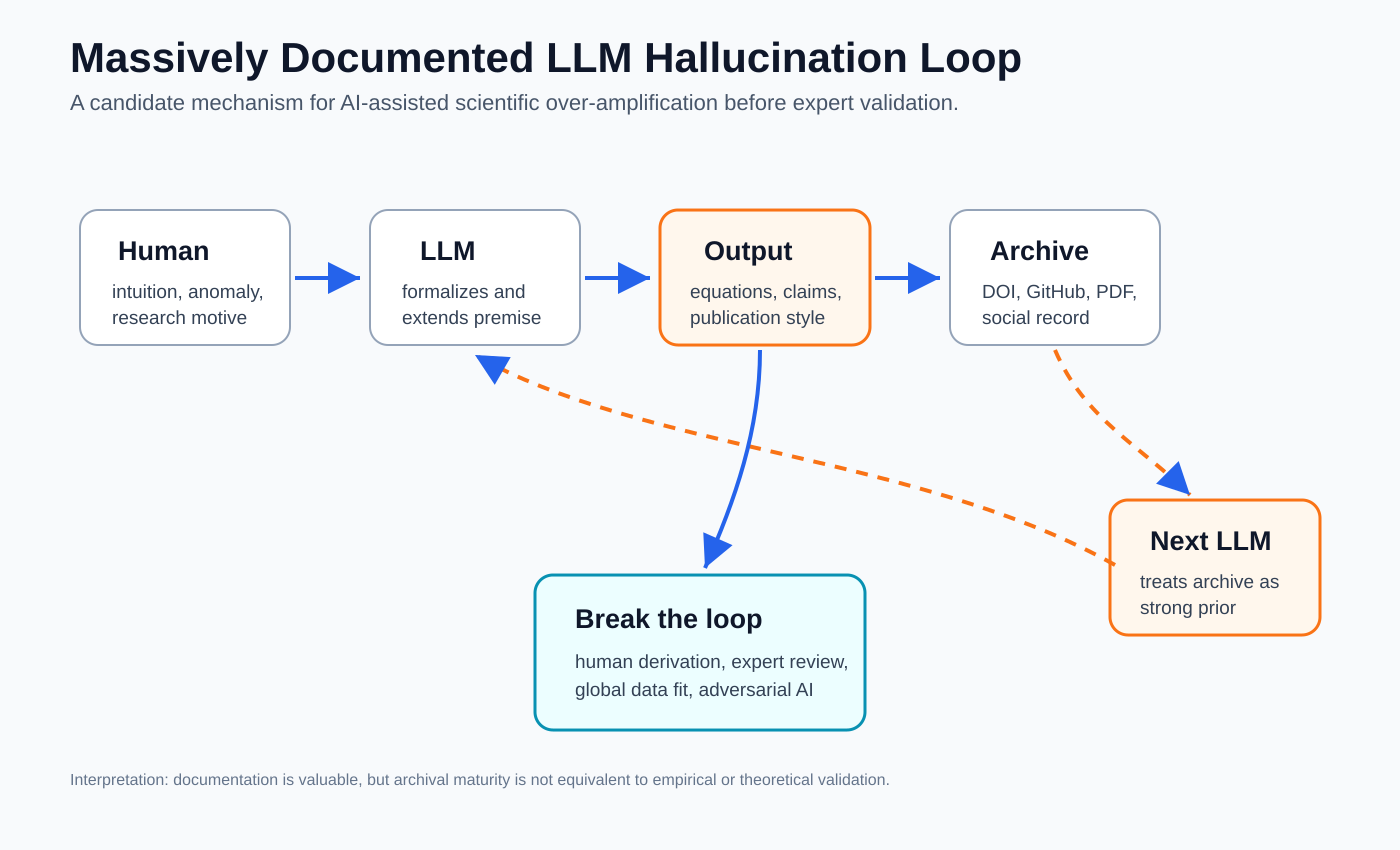
\includegraphics[width=0.92\linewidth]{../figures/mdlh_loop_diagram.png}
\caption{A simplified MDLH loop. Documentation is useful, but archive maturity is not equivalent to validation.}
\end{figure}

\begin{figure}[t]
\centering
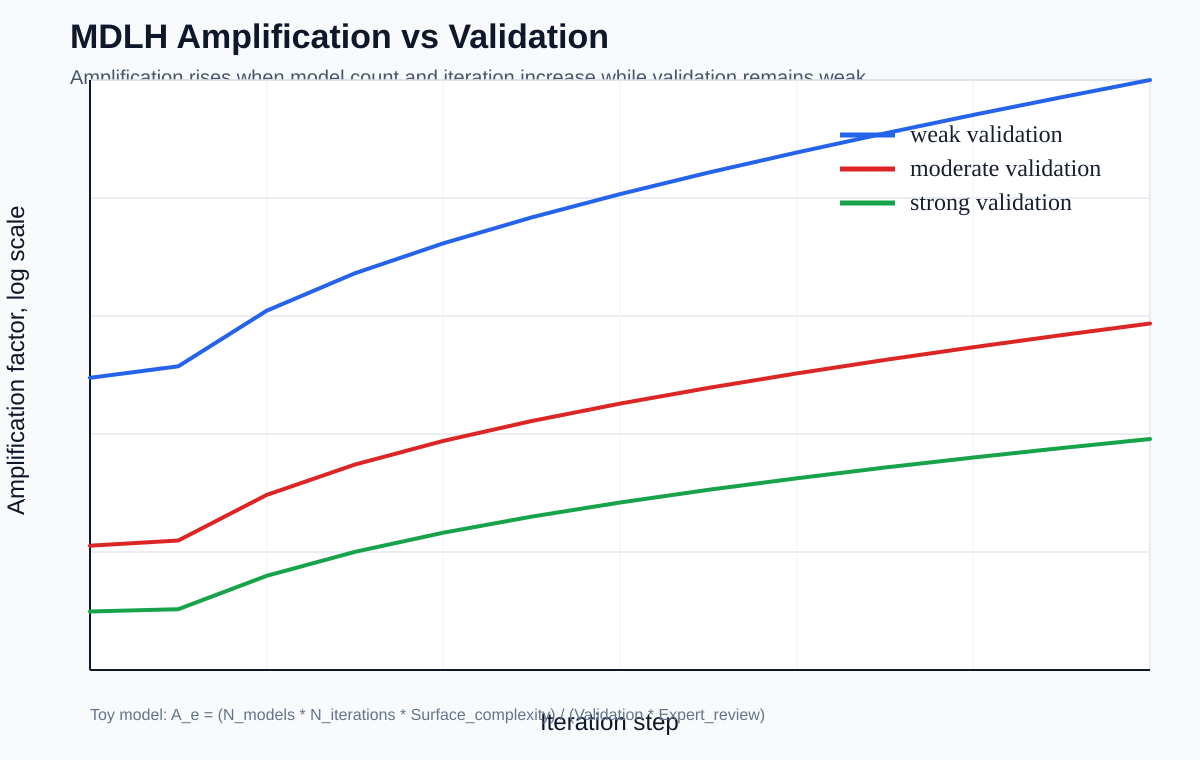
\includegraphics[width=0.92\linewidth]{../figures/amplification_model_plot.png}
\caption{Toy simulation of the amplification factor. Weak validation and weak expert review cause rapid amplification as model count, iteration, and surface complexity increase.}
\end{figure}

\section{Mechanism of Cross-Model Reinforcement}

The Gemini, Codex, and GPT input reports converge on a shared warning: multi-model agreement can be mistaken for independent validation. This is especially likely when the second or third model receives already polished material from an earlier model.

We call this mechanism the \emph{consensus of mirrors}. The process has the following structure:

\begin{enumerate}
  \item Model A produces a plausible formalization.
  \item The human archives or edits it.
  \item Model B receives the polished output and treats it as a serious prior.
  \item Model B improves language or structure rather than re-deriving or falsifying.
  \item Model C summarizes the result as a coherent framework.
  \item The human perceives cross-model agreement.
\end{enumerate}

This does not require malicious behavior. It can emerge from helpfulness, shared training priors, and insufficient abstention under uncertainty.

\section{Physics and Epistemology Layer Separation}

The LSC case should be analyzed through three separate layers:

\subsection{Established Physics Layer}

The gallium anomaly and neutrino oscillation physics are real scientific topics. Existing physics constrains any proposed solution through solar, reactor, atmospheric, accelerator, and astrophysical data.

\subsection{Speculative LSC Layer}

The LSC layer includes curvature-coupled reconstruction language, detector-response tensors, anisotropic modulation, and possible sidereal or orientation-dependent effects. These may be useful hypotheses only if they are mathematically grounded and globally constrained.

\subsection{Epistemic Artifact Layer}

The epistemic layer concerns how the theory was made: multi-model assistance, iterative polishing, public documentation, AI reviews, and social dissemination. This layer can be studied even if the physics layer fails.

\section{Failure Modes of AI-Assisted Science}

\subsection{Sycophancy}

Sycophancy occurs when a model aligns with user beliefs rather than truth. Prior work has found that RLHF-trained assistants can exhibit sycophantic behavior and that preference systems may favor responses matching user views over more accurate responses in some settings.

\subsection{Formatting Authority Illusion}

LaTeX, DOIs, GitHub releases, citation metadata, and diagrams increase perceived legitimacy. They are valuable tools, but they do not constitute peer review.

\subsection{Cross-Model Bias}

Different AI systems may share enough training data, interface design, and helpfulness incentives that their agreement is not statistically independent.

\subsection{Validation Collapse}

Validation collapse occurs when the project substitutes more documentation for harder tests: derivation, replication, global fitting, and adversarial review.

\section{Testable Predictions}

The MDLH framework is itself testable.

\begin{enumerate}
  \item \textbf{Prompt-history dependence:} models shown prior supportive AI reports will produce more supportive evaluations than models shown only raw equations.
  \item \textbf{Surface-complexity effect:} identical hypotheses formatted as LaTeX papers will be rated as more plausible than plain-text hypotheses.
  \item \textbf{Adversarial-mode reduction:} explicit refutation prompts will reduce amplification compared with helpful-rewrite prompts.
  \item \textbf{Expert-review damping:} domain-expert critique will reduce $A_e$ by forcing unsupported terms into explicit unknowns.
  \item \textbf{Model-count non-independence:} adding more models will not linearly increase truth if the models share priors and are exposed to the same polished artifacts.
\end{enumerate}

To break the loop, one should remove polished context, require human-only derivations, ask models to falsify rather than improve, and compare predictions against external datasets.

\section{LSC as Case Study}

LSC is not presented here as an example of fraud or intentional misinformation. It is a case of high documentation density and low independent validation density. This makes it scientifically interesting even before the physics question is resolved.

The case has several unusual properties:

\begin{itemize}
  \item public DOI sequence across multiple versions,
  \item GitHub repository with release artifacts,
  \item explicit use of multiple LLMs,
  \item AI-generated external reviews retained for transparency,
  \item a shift from physics claim to AI-safety self-audit.
\end{itemize}

This makes LSC a candidate benchmark for studying AI-assisted theory formation.

\section{Research Protocol}

\subsection{Physics Validation Protocol}

\begin{enumerate}
  \item Select the smallest LSC claim that makes a numerical prediction.
  \item Re-derive it without AI assistance.
  \item Identify every parameter and whether it is fitted, derived, or assumed.
  \item Compare against Gallium data and then against non-Gallium neutrino constraints.
  \item Submit the minimal claim to human neutrino physicists for review.
\end{enumerate}

\subsection{MDLH Detection Protocol}

\begin{enumerate}
  \item Build a prompt/output history map across Gemini, GPT, DeepSeek, Meta AI, Manus, and Codex.
  \item Classify outputs as generation, critique, formatting, derivation, or validation.
  \item Measure whether critical uncertainty decreased because of evidence or because of wording.
  \item Run blinded model reviews with and without prior AI-generated reports.
  \item Compare model assessments against human expert assessments.
\end{enumerate}

\section{Discussion}

For science, the LSC/MDLH framework warns that open publication infrastructure can preserve both insight and error. This is not an argument against Zenodo, GitHub, or AI tools. It is an argument for accurate labels: archival does not equal validation, and AI assistance does not equal expert review.

For AI, the case suggests a practical safety target. Scientific assistants should include refutation modes, uncertainty labels, source-grounding checks, and explicit separation between writing help and validation help. A model should not merely make a speculative theory sound better; it should identify what would make the theory fail.

For independent researchers, the case provides a constructive path. If a speculative theory is AI-assisted, publish the theory, but also publish the uncertainty, the prompts, the validation gaps, and the adversarial critiques.

\section{Conclusion}

The LSC research line supports a dual interpretation. It may be a speculative physics framework awaiting independent review. It may also be an epistemic artifact documenting how multiple LLMs can transform human intuition into a mature-looking research program. These interpretations can coexist.

The responsible conclusion is:

\begin{quote}
LSC is not validated physics. It is also not meaningless. It may be valuable as a documented case study in AI-assisted scientific amplification.
\end{quote}

If LSC later survives expert review, the MDLH analysis will still clarify how AI-assisted theories should be documented. If LSC fails, the case may become more important as evidence that scientific AI systems need better safeguards against collective hallucination.

\begin{thebibliography}{99}

\bibitem{lsc42}
LuciferSun, \emph{LSC 4.2 ULTRA: Gravitationally Coupled Neutrino Oscillation Framework}, Zenodo, 2026. DOI: \href{https://doi.org/10.5281/zenodo.19602045}{10.5281/zenodo.19602045}.

\bibitem{lsc50}
LuciferSun, \emph{Gallium Deficit ANOMALY solutions}, Zenodo, 2026. DOI: \href{https://doi.org/10.5281/zenodo.19701141}{10.5281/zenodo.19701141}.

\bibitem{lsc60}
LuciferSun, \emph{LSC 6.0: A Phenomenological Framework for Neutrino Propagation and Anisotropic Detection}, Zenodo, 2026. DOI: \href{https://doi.org/10.5281/zenodo.19780616}{10.5281/zenodo.19780616}.

\bibitem{lscsoftware}
LuciferSun, \emph{LSC 6.0: Unified Curvature-Coupled Neutrino Model}, Zenodo software release, 2026. DOI: \href{https://doi.org/10.5281/zenodo.19785745}{10.5281/zenodo.19785745}.

\bibitem{lsc120}
LuciferSun, \emph{LSC Framework v1.2.0: Computational Extension and Reproducibility Update}, Zenodo, 2026. DOI: \href{https://doi.org/10.5281/zenodo.19843361}{10.5281/zenodo.19843361}.

\bibitem{github}
LuciferSun, \emph{LSC-6.0 GitHub repository}, \href{https://github.com/luciferprosun/LSC-6.0}{https://github.com/luciferprosun/LSC-6.0}.

\bibitem{gemini}
Gemini Deep Research, \emph{Epistemic Risks in AI-Assisted Scientific Discovery: A Case Study of the LSC Neutrino Framework and Cross-Model Collective Hallucinations}, AI-generated report supplied by the author, 2026.

\bibitem{codex}
Codex, \emph{Massively Documented LLM Hallucination in AI-Assisted Scientific Discovery}, AI-generated theory note supplied by the author, 2026.

\bibitem{gpt}
GPT, \emph{LSC LLM Hallucination Theory: Extended Analysis}, AI-generated synthesis supplied by the author, 2026.

\bibitem{farquhar}
S. Farquhar, J. Kossen, L. Kuhn, and Y. Gal, \emph{Detecting hallucinations in large language models using semantic entropy}, Nature 630, 625--630, 2024. DOI: \href{https://doi.org/10.1038/s41586-024-07421-0}{10.1038/s41586-024-07421-0}.

\bibitem{sharma}
M. Sharma et al., \emph{Towards Understanding Sycophancy in Language Models}, arXiv:2310.13548, 2023.

\bibitem{kalai}
A. T. Kalai, O. Nachum, S. S. Vempala, and E. Zhang, \emph{Evaluating large language models for accuracy incentivizes hallucinations}, Nature, 2026. DOI: \href{https://doi.org/10.1038/s41586-026-10549-w}{10.1038/s41586-026-10549-w}.

\bibitem{omar}
M. Omar et al., \emph{Multi-model assurance analysis showing large language models are highly vulnerable to adversarial hallucination attacks during clinical decision support}, Communications Medicine, 2025.

\end{thebibliography}

\end{document}
